% !TEX encoding = UTF-8 Unicode
% !TEX TS-program = XeLaTex

\documentclass[
	a0,
	portrait
	]{a0poster}

\usepackage{multicol}
\columnsep=60pt 
\columnseprule=1pt
\def\columnseprulecolor{\color{cyellow}}

\usepackage[svgnames]{xcolor} 

\usepackage{palatino} 

\usepackage{lipsum}

\usepackage{graphicx} % Required for including images
\graphicspath{{img/}} % Location of the graphics files

\usepackage{booktabs} % Top and bottom rules for table
\usepackage[
	font=small,
	labelfont=bf
	]{caption} % Required for specifying captions to tables and figures

\usepackage{
	amsfonts,
	amsmath,
	amsthm,
	amssymb
	} % For math fonts, symbols and environments
	
\usepackage{wrapfig} % Allows wrapping text around tables and figures

\usepackage{tikz}
\usetikzlibrary{
	shapes,
	arrows
	}

\usepackage{float}

\usepackage{color}

\usepackage{
	fontspec,
	xltxtra,
	xunicode
	}

\usepackage[italian]{babel}
	
\defaultfontfeatures{Mapping=tex-text}

\setromanfont[Mapping=tex-text]{Fira Sans}

\setsansfont[
	Scale=MatchLowercase,
	Mapping=tex-text
	]{Fira Sans}
	
\setmonofont[]{Fira Mono}

\definecolor{cpurple}{RGB}{81,69,148} % #514594
\definecolor{cyellow}{RGB}{243,186,68} % #F3BA44

\usepackage{multirow}

\usepackage{booktabs}

\usepackage{tabularx}

\usepackage{titlesec}

\usepackage{lettrine}

\titlespacing*{\section}{0pt}{0\baselineskip}{0.1\baselineskip}
\titlespacing*{\subsection}{0pt}{0\baselineskip}{0.5\baselineskip}

\renewcommand\footnoterule{}

\usepackage{hyperref}
\usepackage{cleveref}

\crefformat{footnote}{#2\footnotemark[#1]#3}

% ------------------------------------ DOCUMENT
  
\begin{document}

\color{cpurple} 

% ------------------------------------ TESTATA

\begin{table}[htp]
\color{cpurple} 
\begin{center}
\begin{tabularx}{\textwidth}{Xc}
\veryHuge \textbf{\color{cyellow}SEAM} & \multirow{ 5}{*}{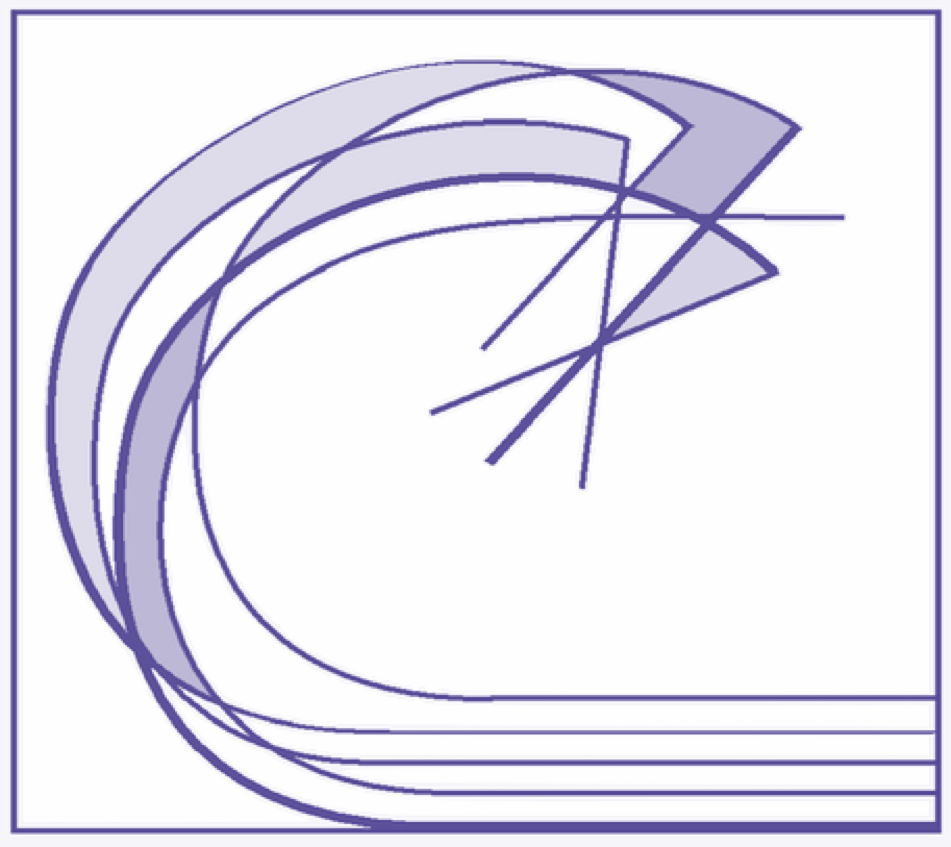
\includegraphics[scale=.35]{Conservatorio-purple.png}} \\
\Huge \textit{Sustained Electro-Acoustic Music} & \\[1.cm]
\huge \textbf{\color{cyellow}Davide Tedesco, Giuseppe Silvi} & \\[0.2cm]
\huge Conservatorio S. Cecilia di Roma & \\[0.2cm]
\Large \texttt{s-e-a-m.github.io} & \\[1.2cm]
\large \textit{Rapporto sui materiali di ricerca di:} & CONSERVATORIO S. CECILIA DI ROMA \\[0.2cm]
\huge  \textbf{\color{cyellow}I'm sitting • Risonanze Erranti • Mobile Locale} &  \\ 
\end{tabularx}
\end{center}
\label{default}
\end{table}%   

\large

% ------------------------------------ ABSTRACT

\noindent La Scuola di Musica Elettronica di Roma ha un ruolo didattico radicato nella tradizione elettroacustica più antica, risalente fino agli albori elettroacustici. Questa verticalità storica non si è mai interrotta e, senza soluzione di continuità, si colloca oggi come fondamento didattico d'eccellenza che pone la scuola del Conservatorio S. Cecilia inevitabilmente in un'ottica sperimentale, di speculazione, ricerca e pratica musicale in linea con il percorso storico. Il percorso didattico-compositivo nell'arco degli studi pone costantemente gli studenti in riflessione con il presente storico, cercando in questa continuità gli stimoli e le prospettive per la costituzione di un'individualità musicale nella piena comprensione del ruolo collettivo che ciò comporta. La produzione artistica degli studenti incontra puntualmente il confronto acustico, percettivo e materico con l'ascolto musicale, spingendoli verso un'autonomia completa e matura. Una ricerca autonoma non ancora supportata ed incoraggiata dalle istituzioni ma che attraverso la rete associativa privata può fare da collegamento tra lo studio ed il mondo del lavoro, come è il caso delle opere qui presentate, prodotte e realizzate al \emph{Centro Ricerche Musicali} per il festival \emph{ArteScienza}. In questa continuità didattico-lavorativa il ruolo dell'Istituzione Conservatorio è un partner essenziale che negli anni è stato capace, muovendosi entro il limiti tipici delle istituzioni italiane, di supportare \emph{EMUFest}, il \emph{Festival di Musica Elettronica di Roma}, stabilendo un legame forte tra didattica e pratica musicale nel luogo di massima fertilità del pensiero musicale che è la sala da concerto.

\normalsize

% ------------------------------------ CORPO

\begin{multicols}{4}

\begin{center}
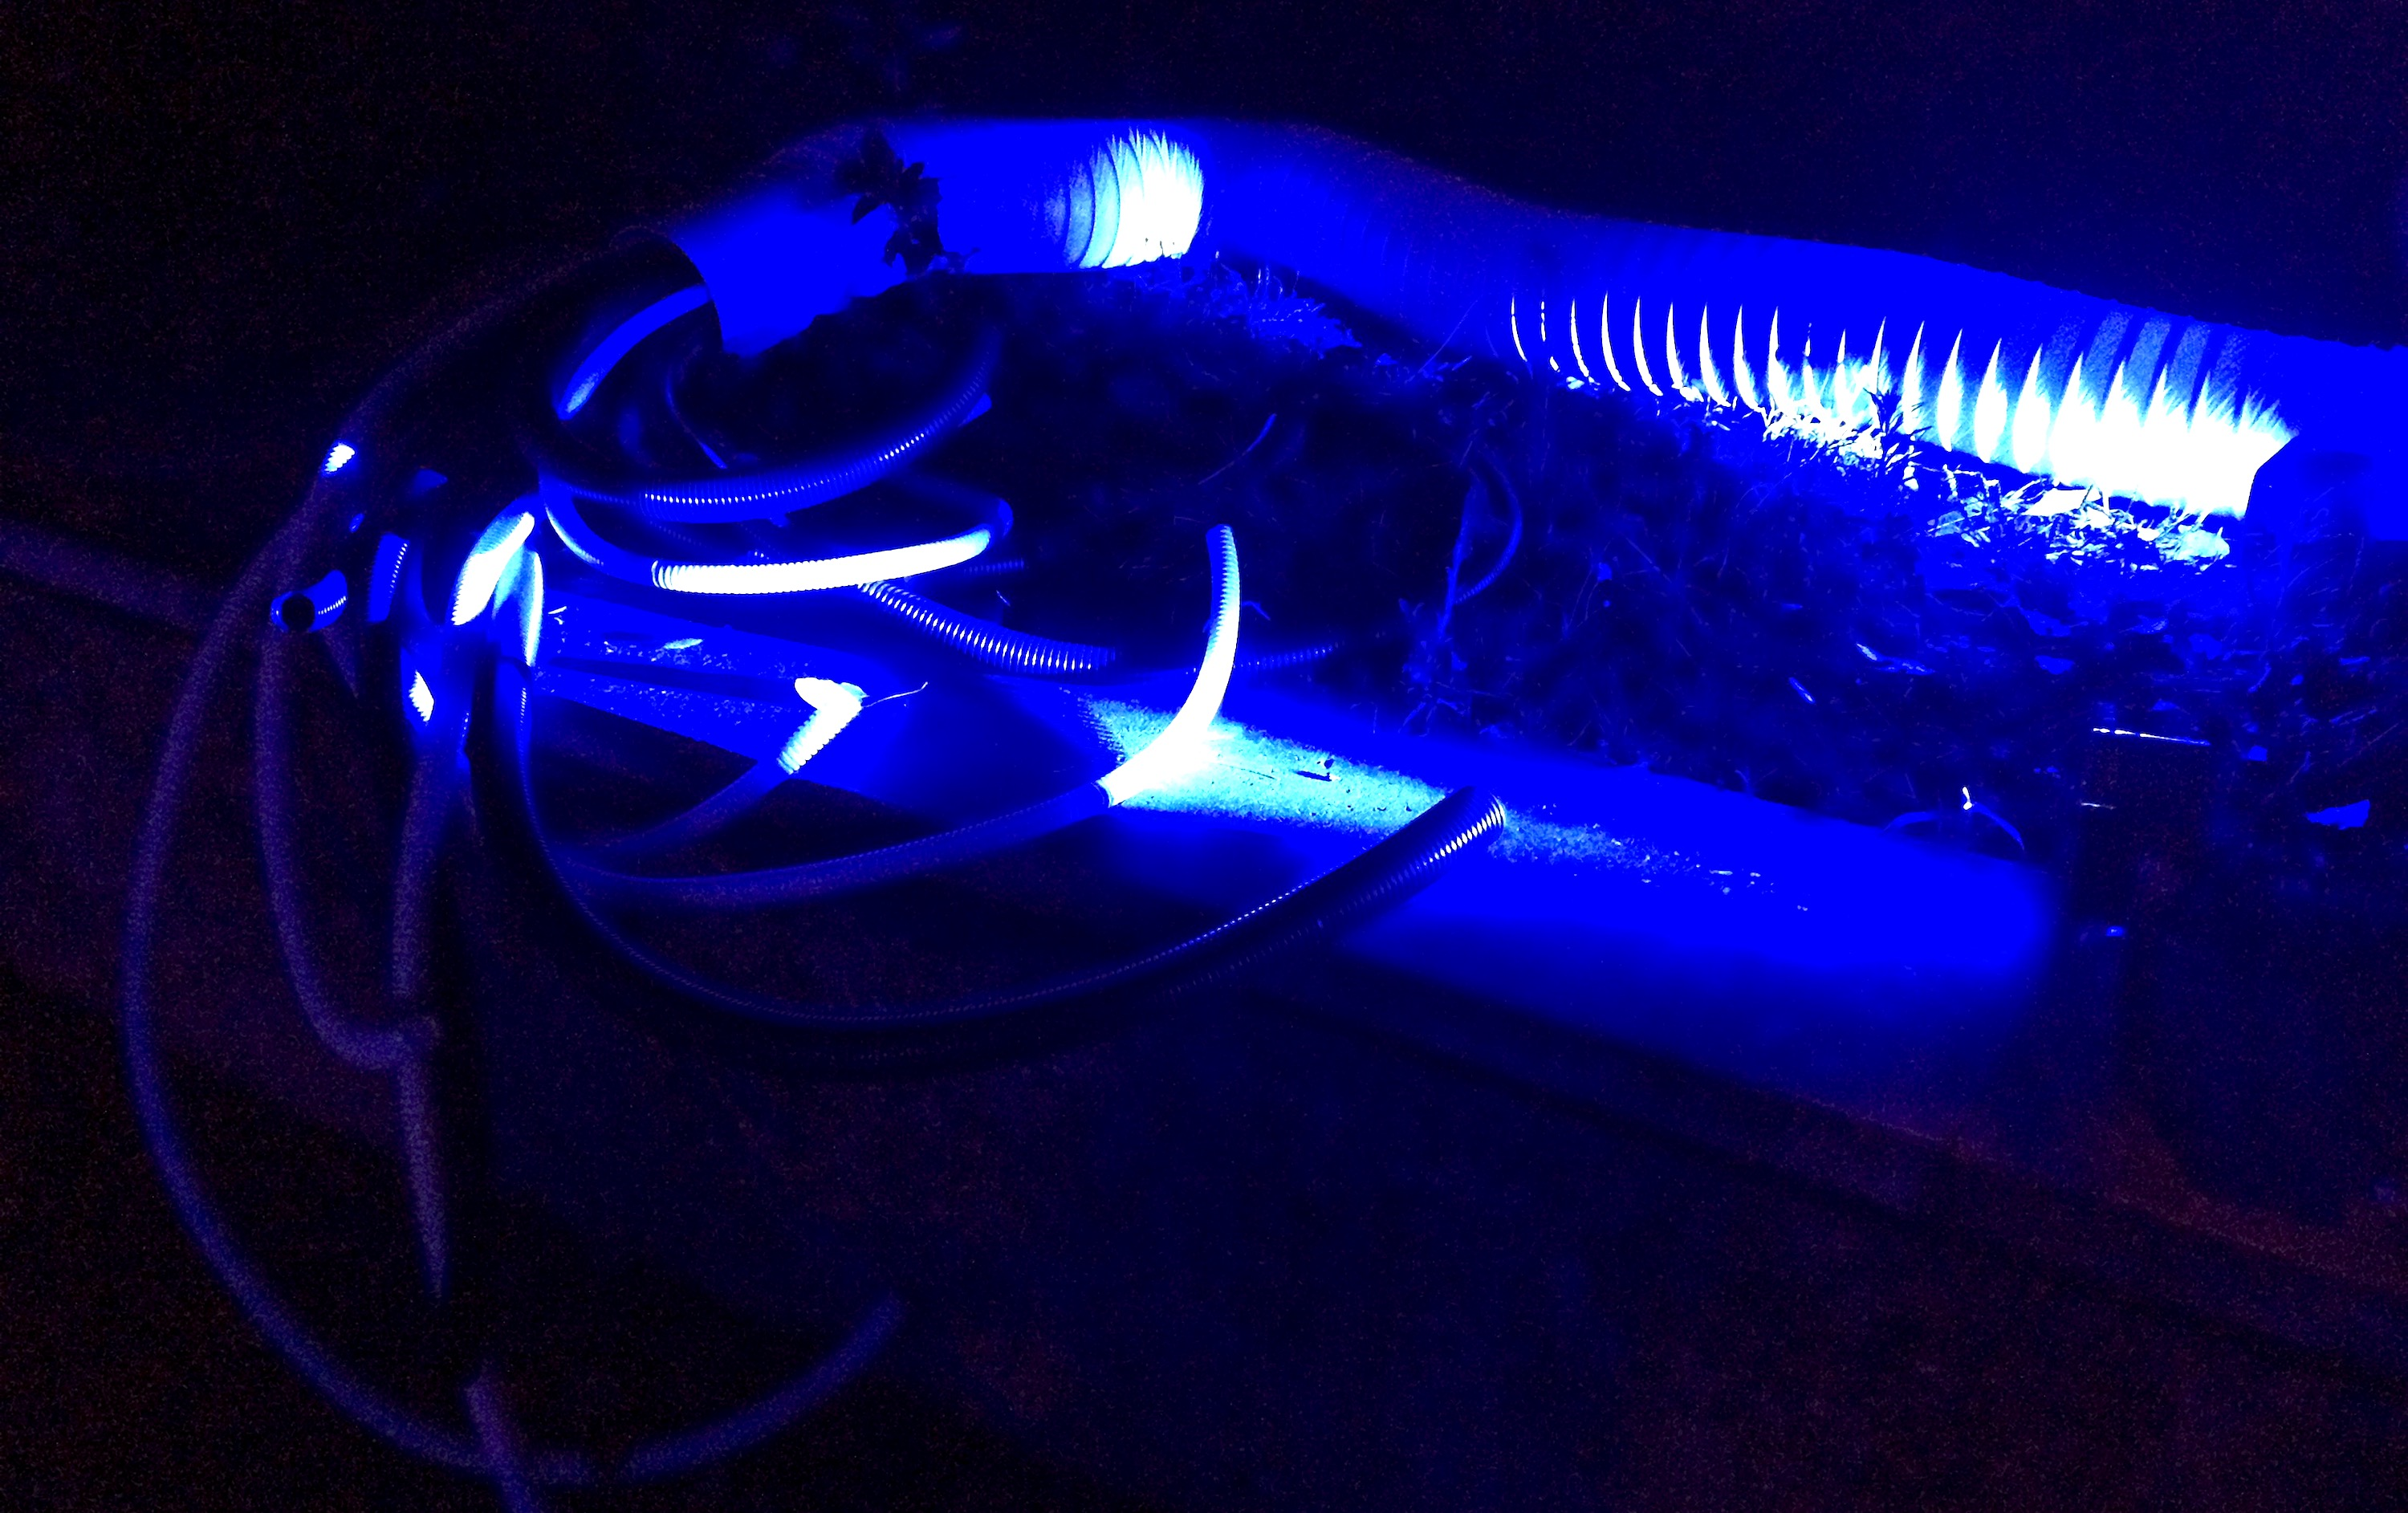
\includegraphics[width=1.\linewidth]{IMG_2143}
\end{center}

% ------------------------------------ ELENA

\section*{\color{cyellow}WRITING}

\lettrine{I'M}{SITTING IN A ROOM} parte dalla definizione di suono come percezione acustica del fenomeno fisico delle oscillazioni delle molecole di un fluido (in questo caso l’aria) rispetto alla loro posizione di equilibrio. L’intento è di creare uno spazio sonoro che descriva questa definizione, dove l’esperienza più naturale possibile del fenomeno può essere data dal semplice ascolto di suono circostante.

Esplorando l’idea dell'aria stessa come meccanismo di eccitazione di sorgenti sonore, \emph{Ainur} sarà costituita da una strumentazione costruita appositamente: cinque ventilatori produrranno aria che farà suonare dei tubi corrugati. Le diverse particolarità di suono dipenderanno dalla varietà di lunghezza e diametro tubi. 

La parte attiva del fruitore all’interno di questo spazio sonoro d’aria avviene proprio sui tubi: il pubblico potrà variare la pressione dell’aria all’interno del ventilatore tramite un’apposita postazione di controllo liberamente accessibile. Risuonano così le frequenze (e i loro armonici) proprie dei tubi, più gravi e deboli a pressione minima e più acute e molto più forti a pressione massima. L’ospite può quindi interagire in modo diretto e consapevole. 

Alla bocca del ventilatore, quindi alla base del tubo sonoro, viene posto un altoparlante che diffonderà delle illusioni di Shepard come sostegno dei suoni nelle frequenze più gravi che i tubi non arrivano a produrre, armonizzando il rumore del ventilatore non solo alle sonorità dei corrugati, ma soprattutto all’ambiente esterno.

L’aspetto estetico scultoreo è in sintonia con il giardino, particolare e curioso\footnote{\label{note1}\color{cpurple} Progetto \emph{Il Giardino dei suoni segreti} sostenuto da \emph{SIAE Sillumina} – \emph{Nuove opere} (\emph{ArteScienza 2017}, Goethe-Institut Rom)}.

\bigskip

\begin{quotation}
\begin{it}
\begin{flushright}
\noindent Allora la voce degli Ainur, quasi con arpe e liuti, e flauti e trombe, e viole e organi, quasi con innumerevoli cori che cantassero con parole, prese a plasmare il tema di Ilùvatar in una grande musica; e si levò un suono di melodie infinitamente avvicendantisi, conteste in armonia, che trascendevano l’udibile in profondità e altezza, e i luoghi della dimora di Ilùvatar ne erano riempiti a traboccarne, e la musica e l’eco della musica si spandevano nel Vuoto, ed esso non era vacuo.
\end{flushright}
\end{it}
\flushright{da \emph{Il Silmarillion},\\J. R. R. Tolkien}
\end{quotation}

\vfill

~

\columnbreak

% ------------------------------------ MARCO

\begin{center}
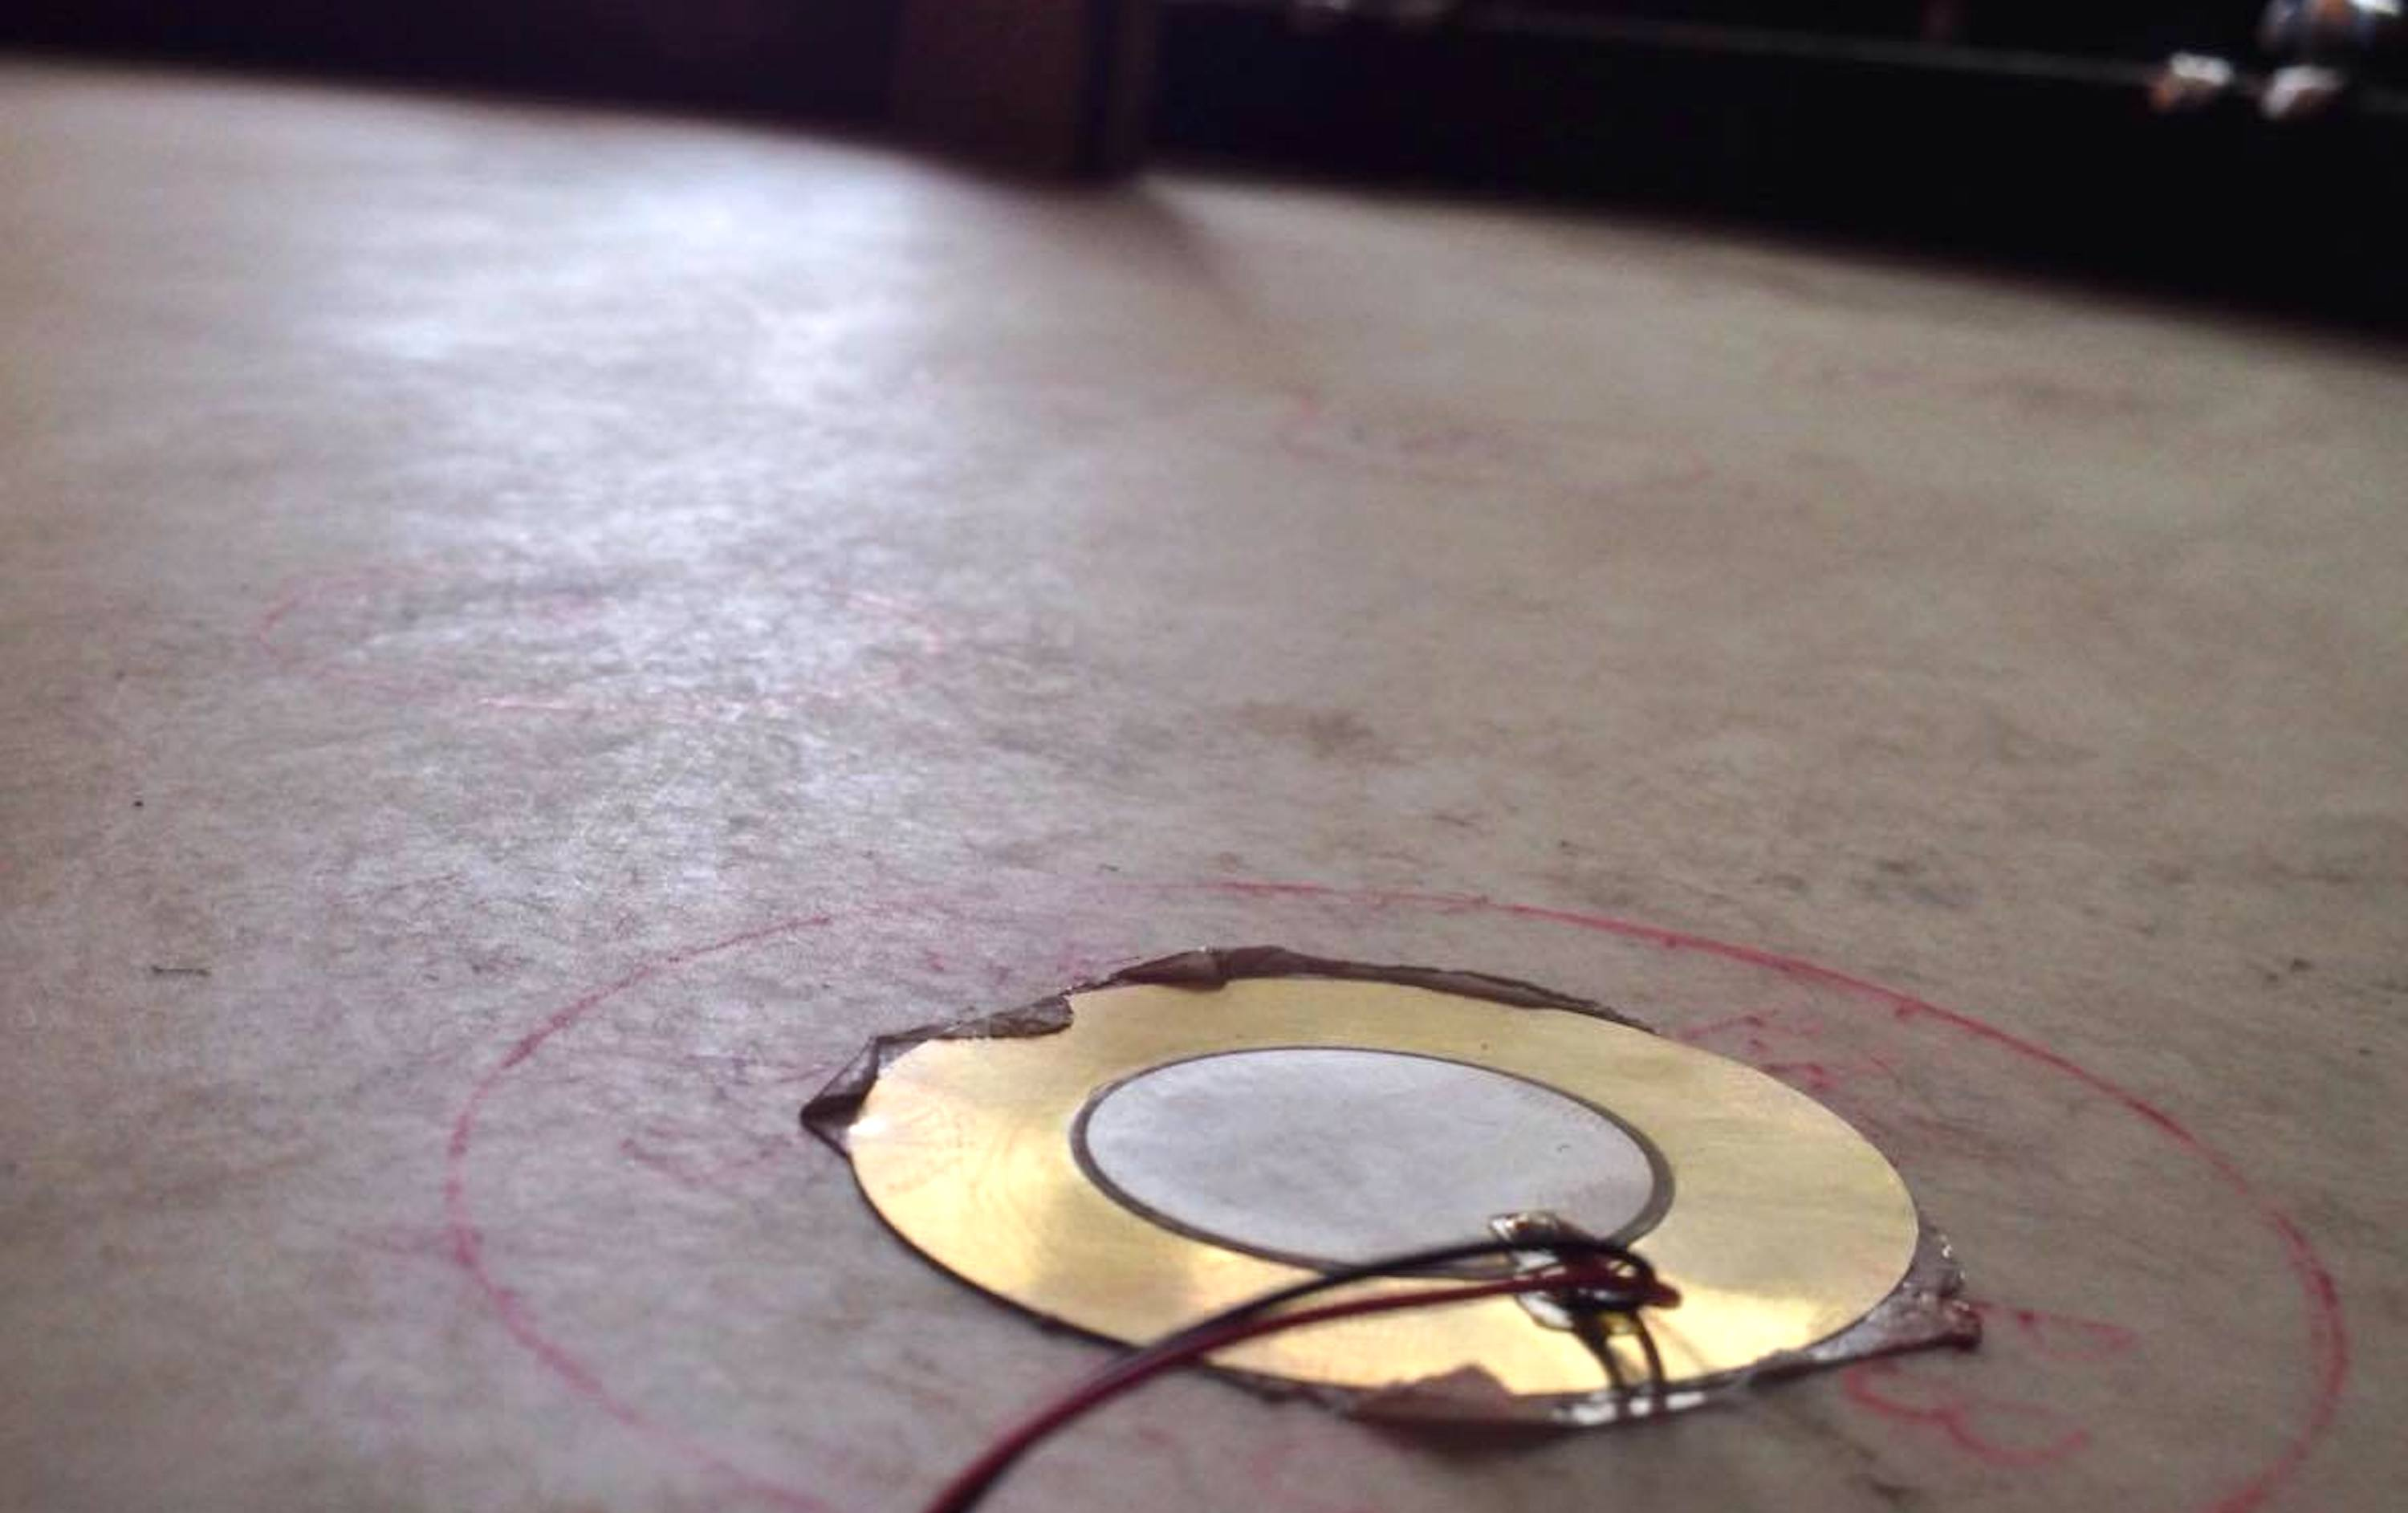
\includegraphics[width=1.\linewidth]{23714923_10155152202522951_954200240_o}
\end{center}

\section*{\color{cyellow}RE-WRITING}

\lettrine{RISONANZE}{ERRANTI}.
La doppia membrana di ognuna delle grancasse sigilla lo spazio in un meccanismo complesso di auto-informazione che si stabilizza nel tempo. È già un sistema che si auto-alimenta fisicamente, portando vibrazioni da una superficie all'altra in un tempo strumentale. Questo meccanismo è amplificato, portato ad estrema reattività, reso dinamico e controllabile mediante l'applicazione di un sistema di contro-reazione del segnale che sfrutti i modi vibrazionali dello strumento. A questo punto l’esplorazione del corpo strumentale ha virato verso una pratica lontana dalla tradizione. Qui, si è generata un’apertura, un percorso che condensa materiale fluido, distante dall’eco ritmico appartenente allo strumento percussivo. 

I modi vibrazionali vengono così amplificati o disturbati portando ai limiti l’instabile natura dello strumento, tracciando un cammino fatto di suoni/soglia, di vibrazioni in continua trasformazione. Le doppie membrane dialogano tra loro sfruttando lo spazio interno, anch'esso aumentato a luogo specifico, vibrante e risuonante, generando un campo sempre-trasformato.

Dialogo interno e dialogo esterno. Il mezzo, lo spazio ed i tre strumenti verso la definizione di un con-testo saturo, a volte di un luogo sospeso: cammino che parte dallo sfregamento del bordo tramite arco, che passa per la preparazione (corde di contrabbasso e arpa), fino ad arrivare al centro della risonanza, il feedback.

Questo grande flusso di eventi è alimentato dell’interprete stesso come altra estensione dello strumento: chinandosi sulla membrana e soffiando all’interno di un piatto propaga il respiro al fusto, generando risonanze/feedback multifoniche. 

I tre centri sono disposti con la massima distanza possibile; la loro collocazione vuole inglobare lo spettatore  e permette di isolare i comportamenti dei singoli centri, ora comunicanti ora soli. Un orientare l’attenzione al singolare-plurale corpo in vibrazione\footnote{\color{cpurple} \emph{ArteScienza 2017}, Teatro Vascello Roma}. 

\bigskip

\begin{quotation}
\begin{it}
\begin{flushright}
\noindent ma il suono senza intervento è magma è mare
\end{flushright}
\end{it}
\flushright{Elio Pagliarani}
\end{quotation}

\vfill

~

\columnbreak

% ------------------------------------ CLAUDIO

\begin{center}
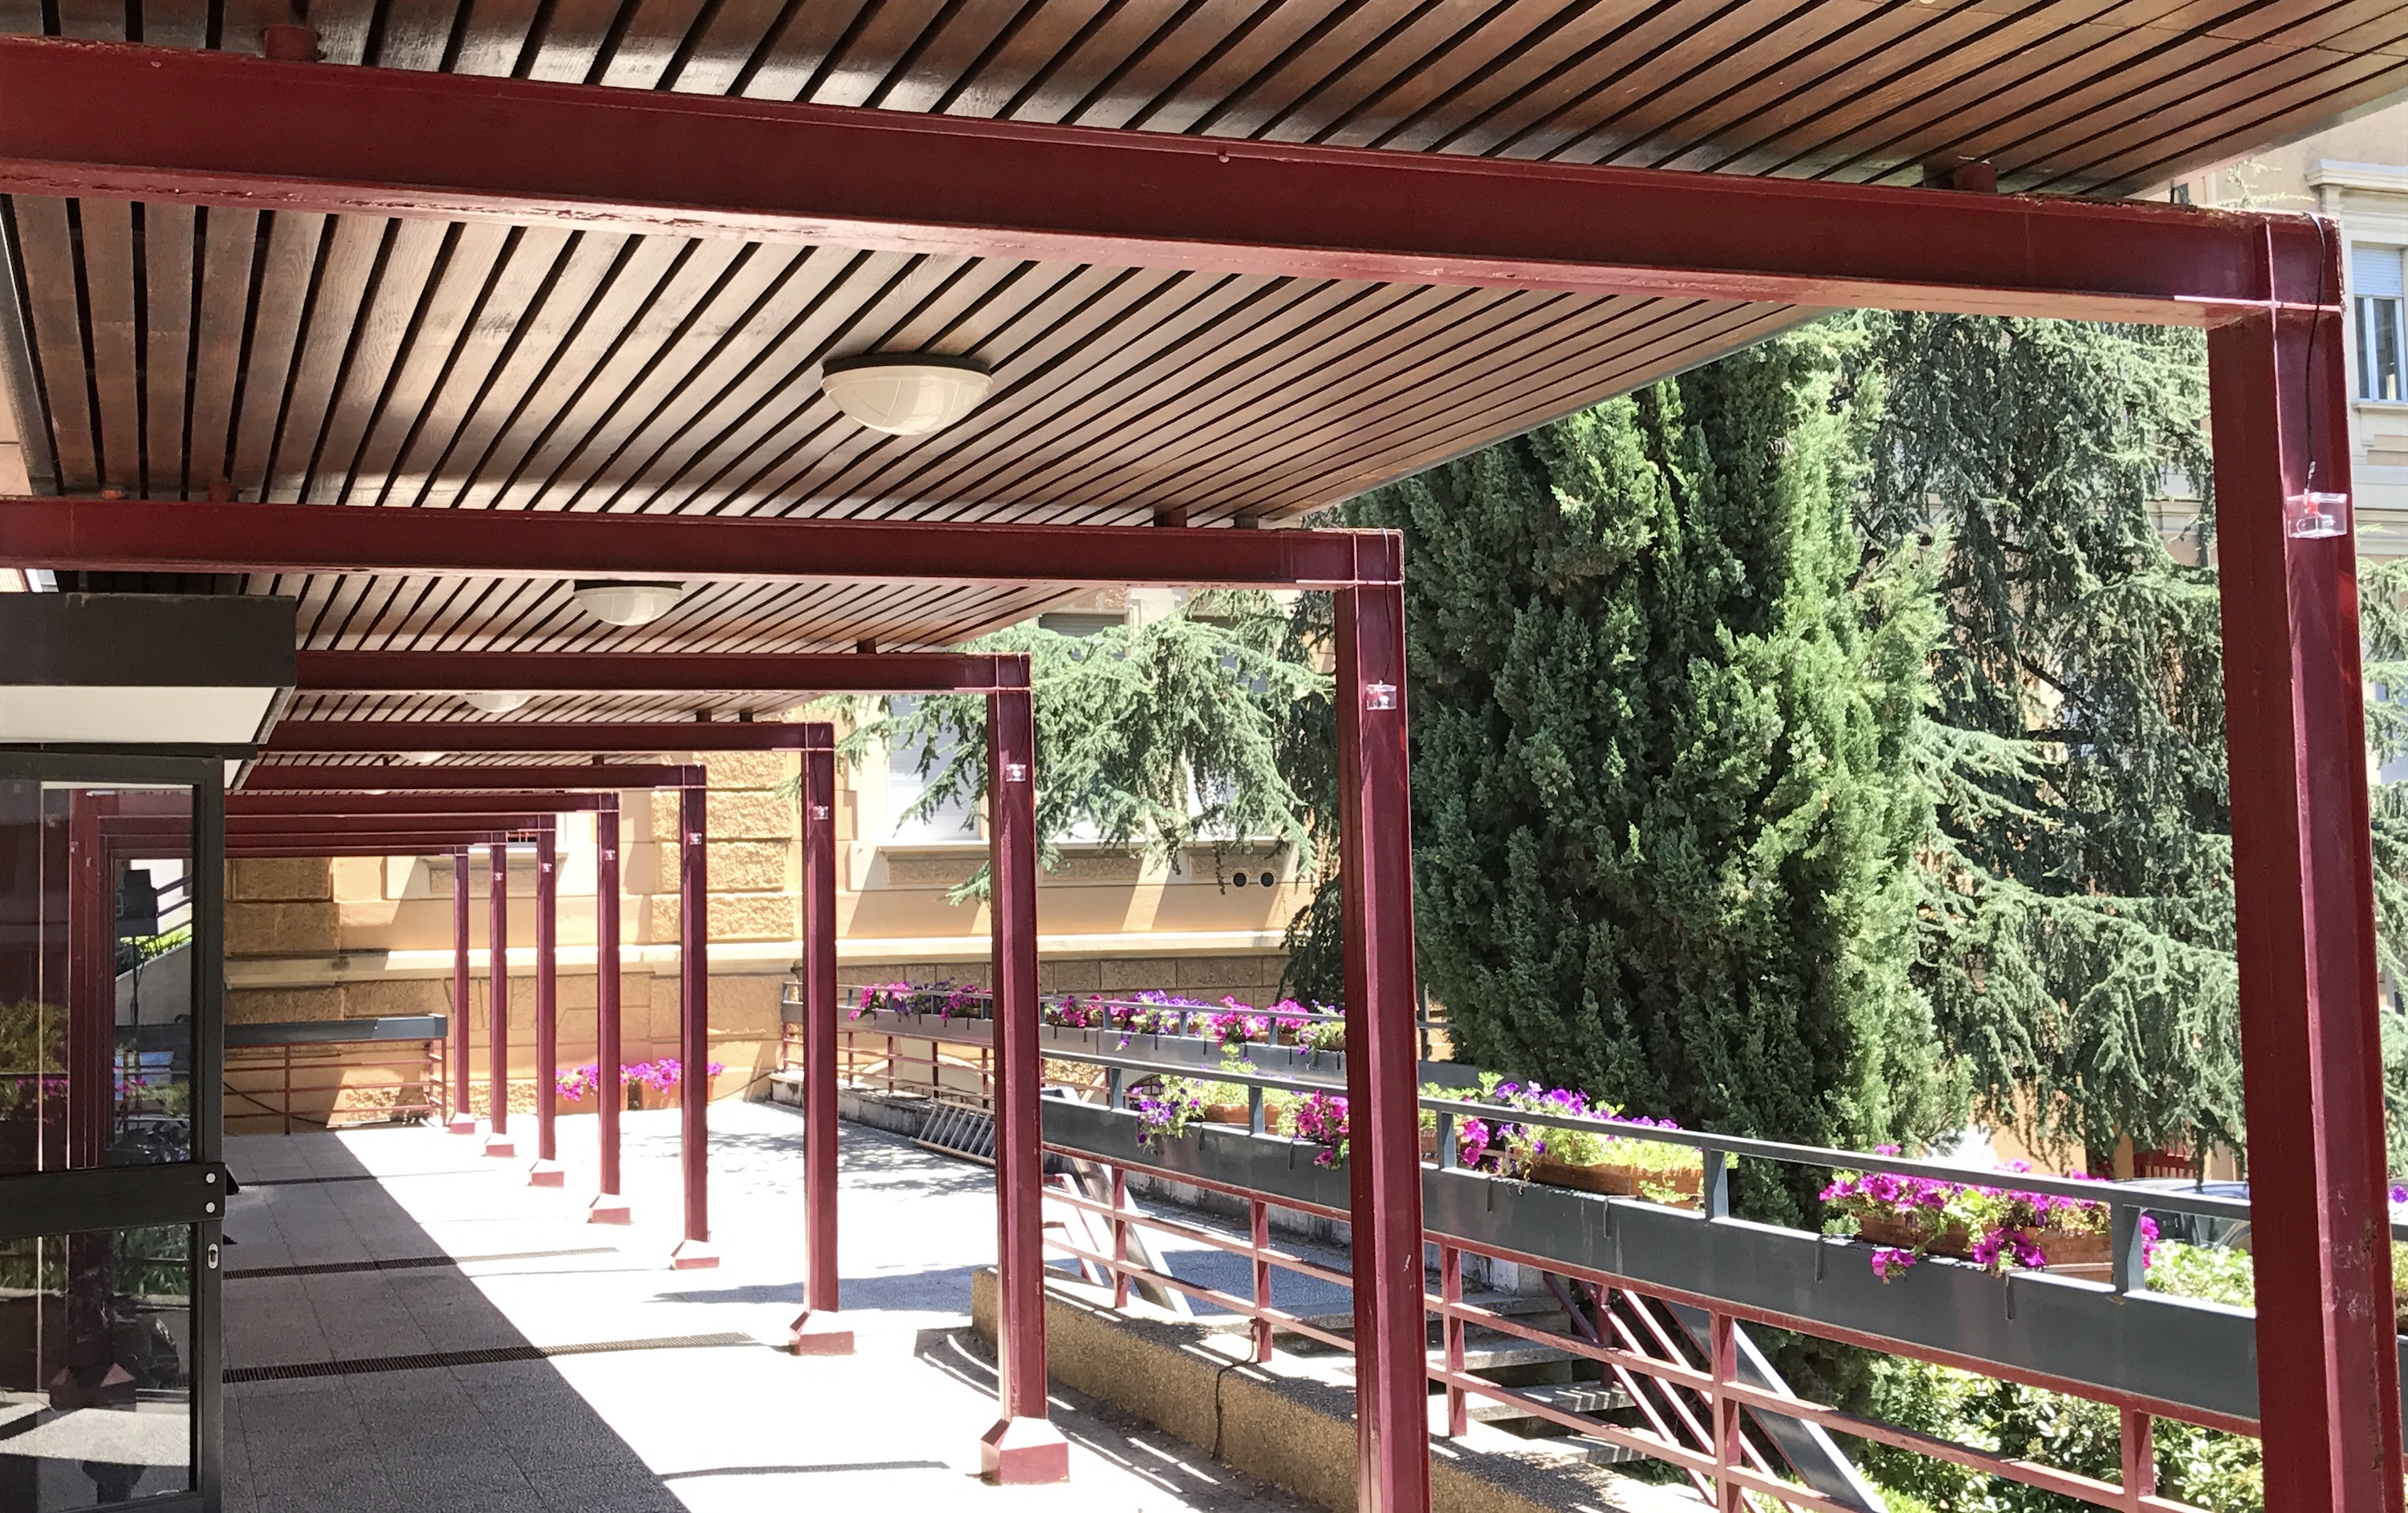
\includegraphics[width=1.\linewidth]{panariello_Solenoidi_sugli_archi}
\end{center}

\section*{\color{cyellow}PORTING}

\lettrine{MOBILE}{Locale} è un’installazione sonora adattiva site specific. Il fulcro del lavoro è mirato a rendere sonoro lo spazio architettonico, permettendo al fruitore di vivere il luogo in maniera acustica, rinnovandone l’interesse in una sorta di percorso sonoro sensibile alla presenza dello spettatore, con il quale l’opera cerca di dialogare, instaurando una connessione tra l’uomo, la macchina e l'ambiente.

Il titolo allude alle cosiddette tre fasi del processo alchemico, inteso nel suo significato più generale e simbolico di conversione e mutazione della materia: Nigredo, Albedo, Rubedo. Decomposizione, Purificazione, Ricomposizione. Fase al Nero, Fase al Bianco, Fase al Rosso.

La prima Fase, la \textbf{decomposizione}, è simboleggiata dagli impulsi che insistono sugli archi del porticato: singoli click sonori distribuiti su tutto il percorso alludono al dissolvimento della materia metallica di cui gli archi sono composti.

Rappresenta l’inizio del percorso tripartito che costituisce l’opera, nel quale avviene migrazione concettuale dallo spazio visivo a quello acustico: il pubblico, viene investito da nuvole di impulsi che contrappongono la loro discontinuità alla continuità della materia di cui l'ambiente è composto. Si crea immediatamente un’articolazione dialettica tra i due domini – vista e udito – in cui uno frattura l’altro: decomposizione.

La seconda Fase, la \textbf{purificazione}, è simboleggiata da due microfoni che capteranno gli eventi sonori per sottoporli ad un processo di autoregolazione. Essi agiscono selettivamente sull’ambiente andando ad individuare quelli che sono realmente gli elementi importanti per l’opera. La capacità di scegliere quali elementi vadano conservati e quali vadano scartati rende il sistema molto versatile ed interessante, più propenso ad adattarsi alle perturbazioni.

La terza Fase, la \textbf{ricomposizione}, è quella nella quale il risultato della precedente elaborazione viene trasformato in nuovi impulsi architettonici, chiudendo un circolo e allo stesso tempo riavviandolo.

L’opera risponde alle sollecitazioni ambientali, imprevedibili, ma per evitare una deriva dell’installazione sono state imposte alcune regole a livello locale, e queste sono quelle che gestiscono la ricomposizione\cref{note1}.

\vfill

~

\columnbreak

% ------------------------------------ MICHELE

\begin{center}
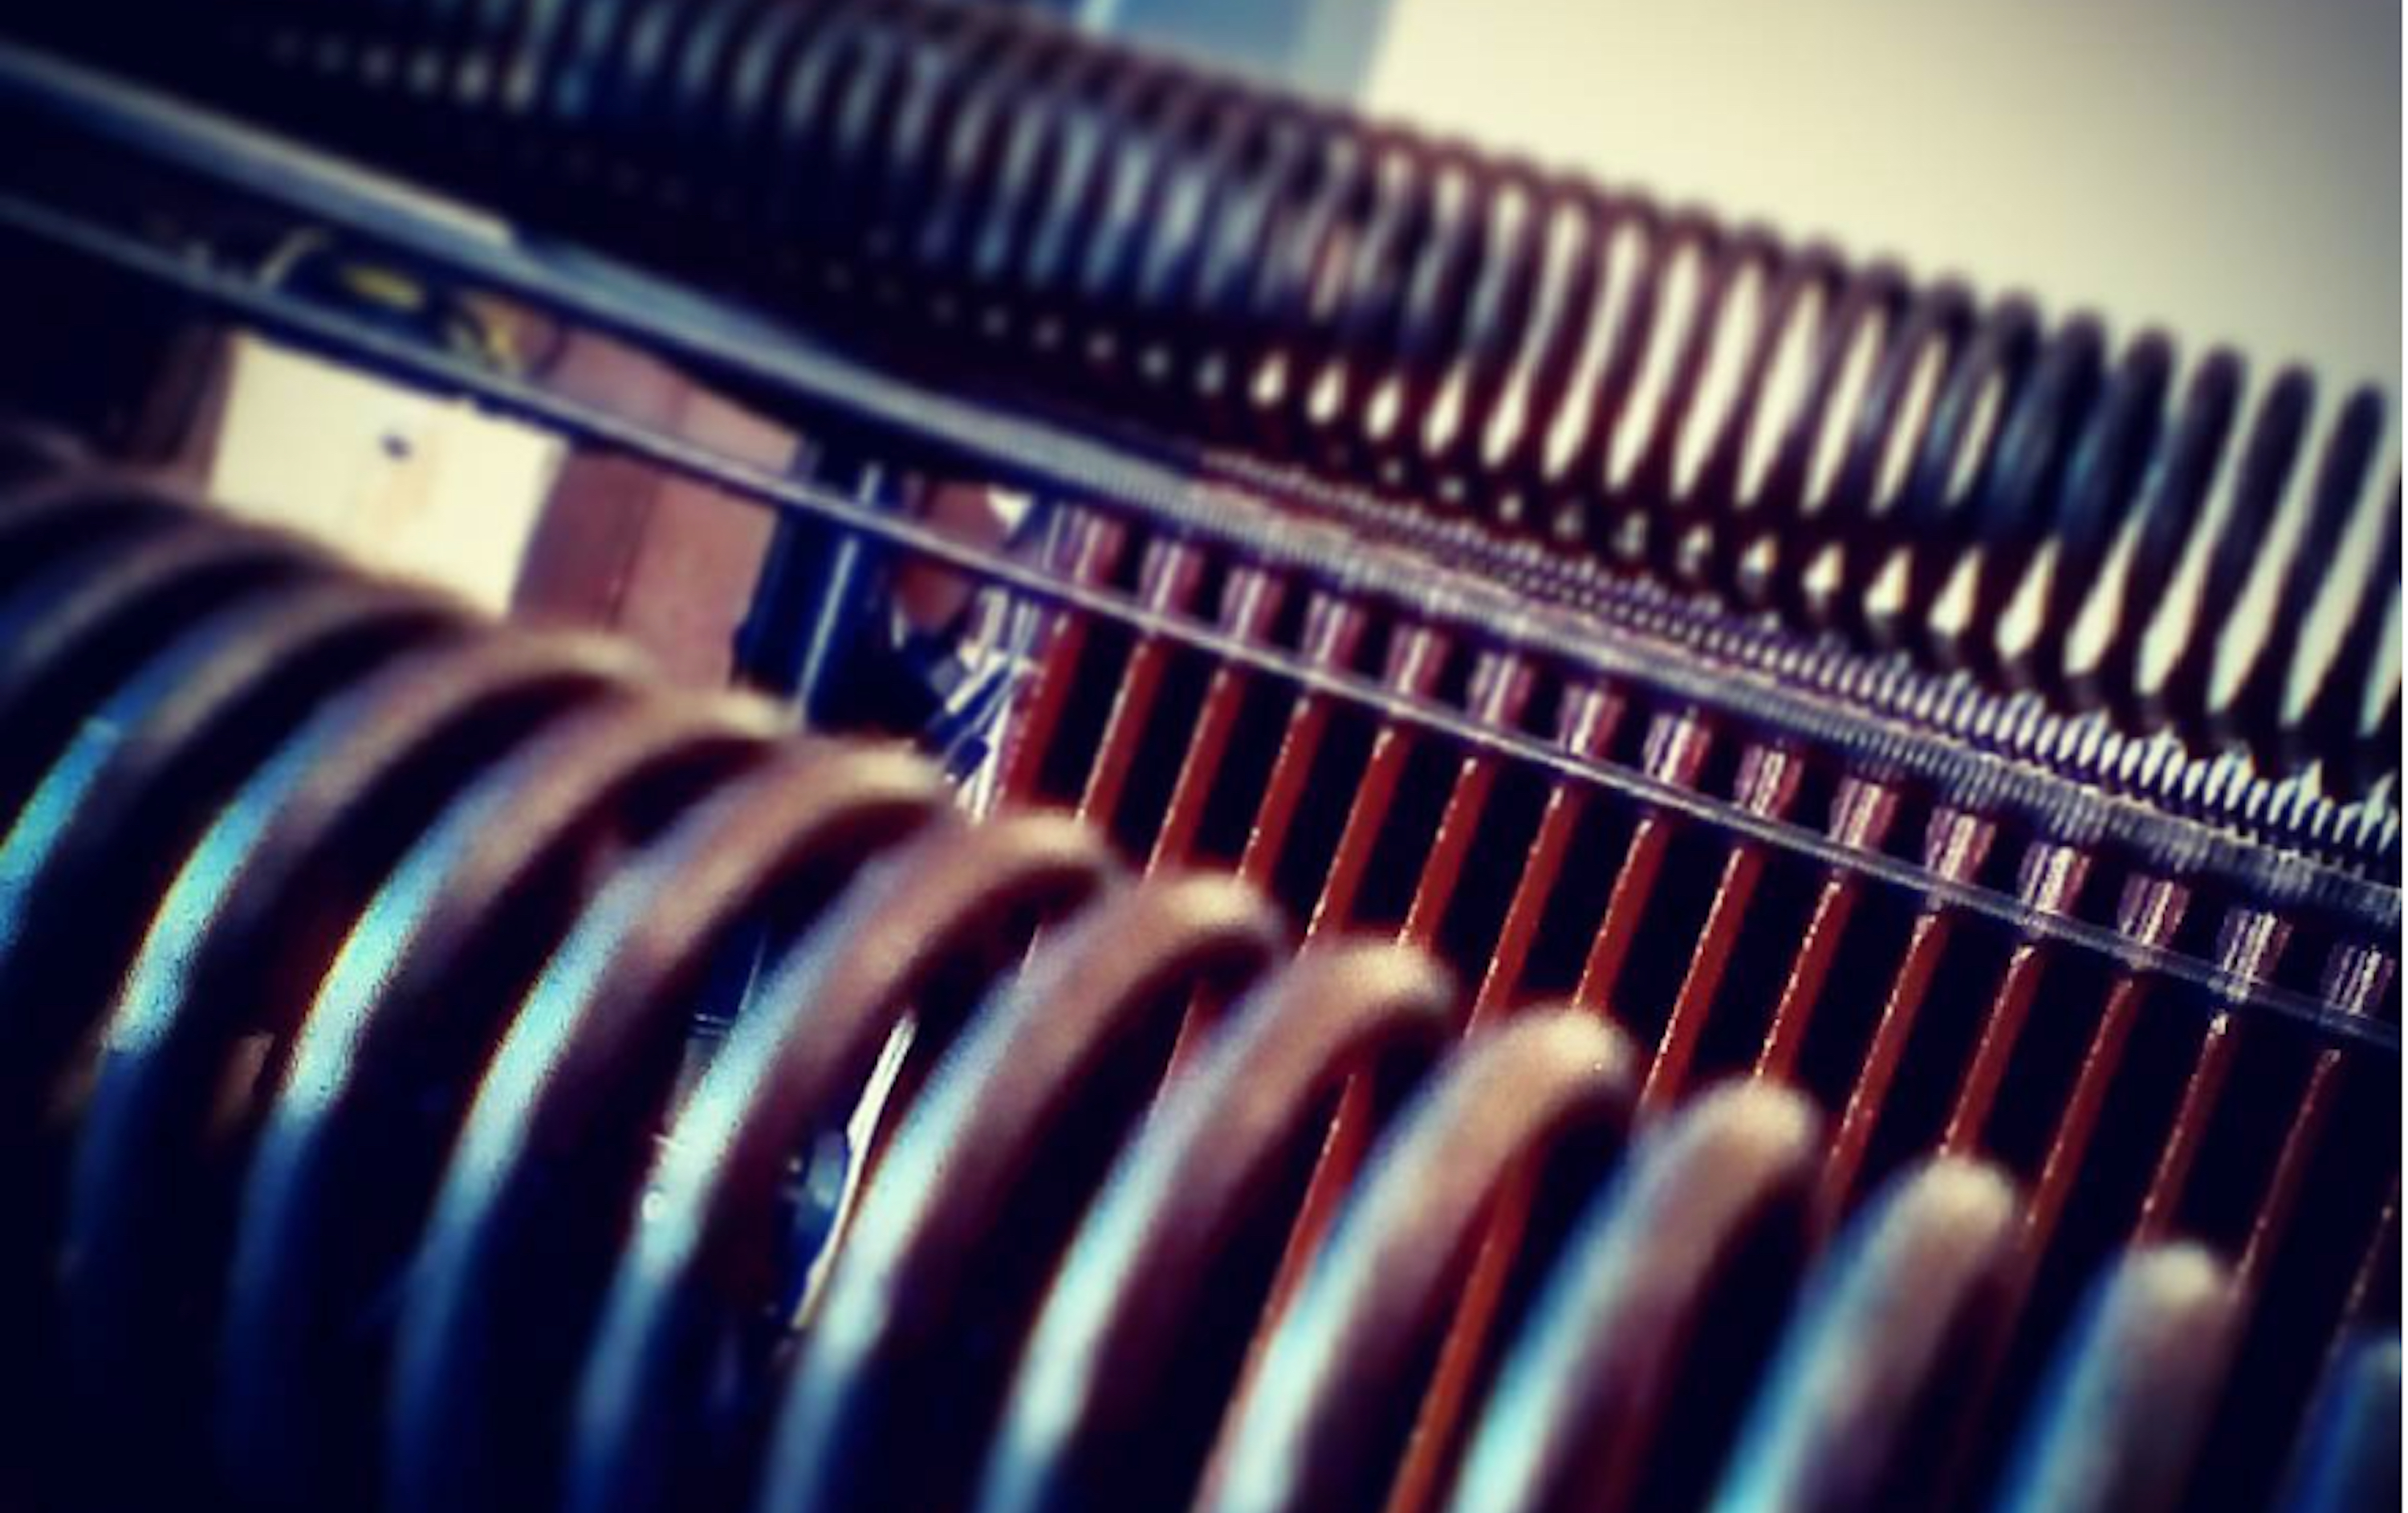
\includegraphics[width=1.\linewidth]{spire}
\end{center}

\section*{\color{cyellow}LIBRARIES}

\lettrine{SEAM}{.lib} \emph{Come un rosone nel cuore di un tempio immenso} è una composizione musicale che porta a compimento una fase del percorso di ricerca su un nuovo strumento elettroacustico.

\emph{Sp.i.r.e.}, acronimo di \emph{Springs Installation Regulated \& Electrified}, fa riferimento alla fisicità del materiale che compone lo strumento. Ogni molla (spring), infatti, è formata da spire e il loro numero rende possibile, a seconda del materiale con il quale vengono eccitate, l’attivazione di armoniche e/o sub-armoniche. La parola electrified indica la componente elettroacustica. L’oggetto sonoro è la metafora de \emph{I Vetri di suono}, la componente elettronica lo rende strumento, mentre, la tipologia di amplificazione e di filtraggio spingono il suono verso l’alto.

La meccanica, l’elettronica e i suoni analogici, rendono possibile la creazione di un mondo nuovo. Vengono a formarsi più dimensioni d’ascolto e più dimensioni tattili, causate dalle diverse risposte d’eccitazioni del materiale. A questa dimensione d’ascolto si unisce la ripresa microfonica, che, nel caso di \emph{Vitres de Son}, sarà omnidirezionale e renderà possibile la riproduzione di tutto il panorama d’ascolto. \emph{Sp.i.r.e.} respira ed emana il segnale elettroacustico in almeno due dimensioni d’ascolto:

\begin{enumerate}
	\item Analogica, la risposta del materiale relativa ai suoni sintetici e al tocco umano
	\item Elettrica ed elettronica, che prende vita grazie ai suoni di sintesi diffusi dagli attuatori
\end{enumerate}

Ogni rigo della partitura è correlato ad un verso dell’omonima poesia di \textbf{\mbox{Antonin} \mbox{Artaud}}. Il sottotitolo è invece un verso della poesia \emph{In Sogno}, e indica la forma nella quale è inscritta la diffusione\footnote{\color{cpurple} \emph{ArteScienza 2018}}. 

\bigskip

\begin{quotation}
\begin{it}
\begin{flushright}
[...] come un rosone nel cuore \\ di un tempio immenso.

E là ascolteremo la cadenza immortale

delle linee e dei corpi ritmati

e di gotiche balaustre profumate

dalla dolcezza dei corpi amati

dagli uomini con grandi anime cadenzate,

dai poeti profumati
\end{flushright}
\end{it}
\flushright{Antonin Artaud}
\end{quotation}

\vfill

~

\end{multicols}
\end{document}